\section{Lösungskonzept}
\label{sec:lösungskonzept}
Die \cref{fig:hwoverview} bietet ein Überblick über den verschiedenen Hardware-Komponenten, die für den \gls{turklingelanlage} notwendig sind. 
\\
Es werden nun zwei Begriffe erklärt, die in diesem Dokument von grosse Bedeutung sind. Das erste ist die \gls{turklingelanlage}. Damit gemeint ist die Gesamtheit der Komponenten die denn Zusammen den Endprodukt darstellen.
\\
Das zweite Begriff ist die \gls{aussensprechstelle}. Wie in der \cref{fig:hwoverview} ersichtlich handelt sich hauptsächlich um ein Mikrocontroller mit verschiedene Modulen die an den Eingangstüre installiert wird.
\\
Räumlich von der \gls{aussensprechstelle} getrennt befindet sich der Server. Diese besteht aus ein Mikrocontroller, die als Server im Einsatz ist, ein Switch die dazu dient die \gls{aussensprechstelle} mit Strom und Datenverbindung zu versorgen und die Relais welche den Türöffner und Glocken betätigen.
\begin{figure}[htb!]
	\begin{center}
		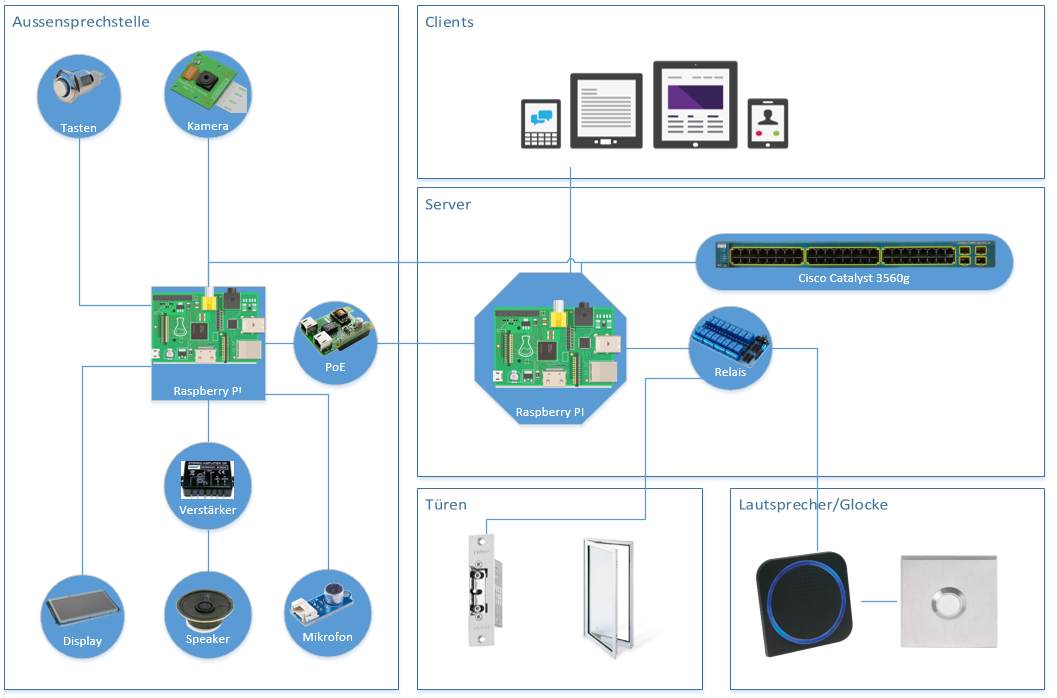
\includegraphics[width=0.95\textwidth]{hwoverview}
		\caption[Hardware Ecosystem]{Hardware Ecosystem}
		\label{fig:hwoverview}
	\end{center}
\end{figure}
\\
Das System wird nicht nur aus Hardware bestehen, sondern auch aus viel Software-Elemente die zusammen arbeiten werden. Als erstes, wie in der Projektplanung bereits definiert, wird die Hardware Seite der Lösung realisiert. Sobald alle Hardware Komponenten getestet und auf Kompatibilität geprüft sein werden, wird die Programmierung stattfinden.

\section{Hardware}
\label{sec:chapterexample}
\subsection{Komponenten}
Das System wird Hardwareseitig hauptsächlich in zwei Teile unterteilt. Der Server und die \gls{aussensprechstelle}.
\\
Die \cref{tbl:SrvHW} und die \cref{tbl:DoorHW} zeigen die benötigten \gls{hw}-Komponenten, welchen an die jeweilige Stellen benötigt werden.
\\
Um den Überblick über die Kosten aller Hardware-Komponenten zu behalten, sind hier auch die Preisen aufgelistet. Wichtig hier ist sicherzustellen, dass die gesamten Hardwarekosten diejenigen der von der Konkurrenz angebotenen Produkte nicht übersteigen.
\\
Die Preise können natürlich leicht abweichen da es sich um Standardkomponenten handelt und die Preise sich schnell ändern. Die Summen sind mehr als Kostenschätzung zu betrachten.

\begin{table}[]
	\centering
	\label{my-label}
	\begin{tabular}{l|ll}
		\multicolumn{1}{r|}{} \textbf{Anzahl} & \textbf{Komponent} \hspace{180pt} & \textbf{Preis} 	\\ \hline
		1	&	Raspberry Pi 3 Model B						& 50.-				\\ \hline
		1	&	Raspberry Gehäuse und Netzteil				& 25.-			\\ \hline
		2	&	8-Kanal Relais Modul						& 15.-			\\ \hline
		1	&	\textit{Kleinmaterial}						& 15.-			\\ \hline
		\textbf{Total}	&									& \textbf{140.-}			\\ \hline
	\end{tabular}
	\caption{Server \gls{hw} Komponenten}
	\label{tbl:SrvHW}
\end{table}

\begin{table}[]
	\centering
	\label{my-label}
	\begin{tabular}{l|ll}
		\multicolumn{1}{r|}{} \textbf{Anzahl} & \textbf{Komponent} \hspace{180pt} & \textbf{Preis} 	\\ \hline
		1	&	Raspberry Pi 3 Model B		   				& 50.-			\\ \hline
		1	&	4" Bildschirm								& 64.-			\\ \hline
		1	&	Raspberry Kamera							& 59.-			\\ \hline
		1	&	\gls{poe} Adapter									& 50.-			\\ \hline
		3	&	Schalter									& 25.-			\\ \hline
		1	&	Mikrophon									& 12.-			\\ \hline
		1	&	Lautsprecher								& 9.-			\\ \hline
		1	&	Audio Verstärker							& 10.-			\\ \hline
		1	&	\textit{Kleinmaterial / Gehäuse}			& 50.-			\\ \hline
		\textbf{Total}	&									& \textbf{329.-}			\\ \hline
	\end{tabular}
	\caption{Aussensprechstelle \gls{hw} Komponenten}
	\label{tbl:DoorHW}
\end{table}

\subsection{Stromspeisung}
\label{sec:poe}
Ein Ziel unser Lösung ist die Installationskosten zu senken und die Montage zu vereinfachen. Aus diesem Grund war für unsere Lösung wichtig, Power over Ethernet zu verwenden.
Moderne Hausalte werden meistens mit Ethernet Verkabelung verlegt. Dank \gls{poe} ist nur noch ein Kabel notwendig, welches Strom und Konnektivität gewährleistet.
\\
\\
Zusätzlich würde das System noch eine Leitung, um den Türöffner zu steuern.
Auch hier kann das Endinstallation vereinfacht werden. Anstatt ein dediziertes Kabel zwischen Server und Türöffner einzuziehen, werden zwei Drähte von dem bereits installierten Ethernet Kabel verwendet.
\\
\\
Cisco Catalyst 3560g welcher für den \gls{poe} Stromversorgung zuständigt ist, verwendet das Phantomspeisung oder Mode A. Das heisst, dass die mit Datenübertragung belegten Drähte mit der Stromversorgung überlagert werden. Das ist möglich da Elektrizität mit eine Frequenz von 60 Hz schwingt und die Datenübertragungen im bereich 10-100MHz liegen.
\begin{figure}[htb!]
	\begin{center}
		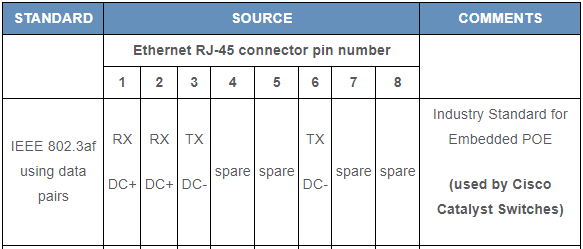
\includegraphics[width=0.89\textwidth]{CatalystPoEpinouts}
		\caption[Catalyst Pinouts]{Catalyst 3560g \gls{poe} Pinbelegung}
		\label{fig:catalystPinouts}
	\end{center}
\end{figure}
\\
Wie im \cref{fig:ethernetBelegung} dargestellt werden die Adern 7 und 8 dazu verwendet um der Türöffner zu betätigen. Aus den 3 verbliebenden Adernpaare kann maximal die Ethernet Kategorie 100BASE-T erreicht werden. Da aber \gls{webrtc} eine erhebliche kleinere Bandbreite in Anspruch nimmt, stellt für die \gls{aussensprechstelle} kein Hinderniss dar.

\begin{figure}[htb!]
	\begin{center}
		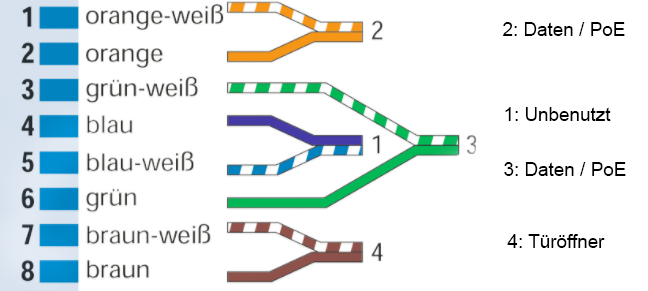
\includegraphics[width=0.89\textwidth]{EthernetPinbelegung}
		\caption[EthernetPinbelegung]{Cat. 7 Ethernet Pinbelegung für die \gls{aussensprechstelle}}
		\label{fig:ethernetBelegung}
	\end{center}
\end{figure}



\subsection{Server}
\label{sec:chapterexample}

Der Server wird mit einem Relay-Board verbunden. Diese wird die Gongs und die Türöffner bedienen. An dieser Stelle ist die Hardware-Konfiguration sehr einfach. Mit der jetzige Hardwarekonfiguration könnten bis auf 8 Wohnungen und 8 Aussensprechstellen angeschlossen werden. Die \cref{fig:pipins} und die \cref{fig:boardpins} zeigen die Pinbelegung auf den Pi und auf dem Relay-Board. Die \cref{tbl:pinroutes} zeigt wie die verschiedene Pins miteinander angeschlossen werden.

\begin{figure}[htb!]
	\begin{center}
		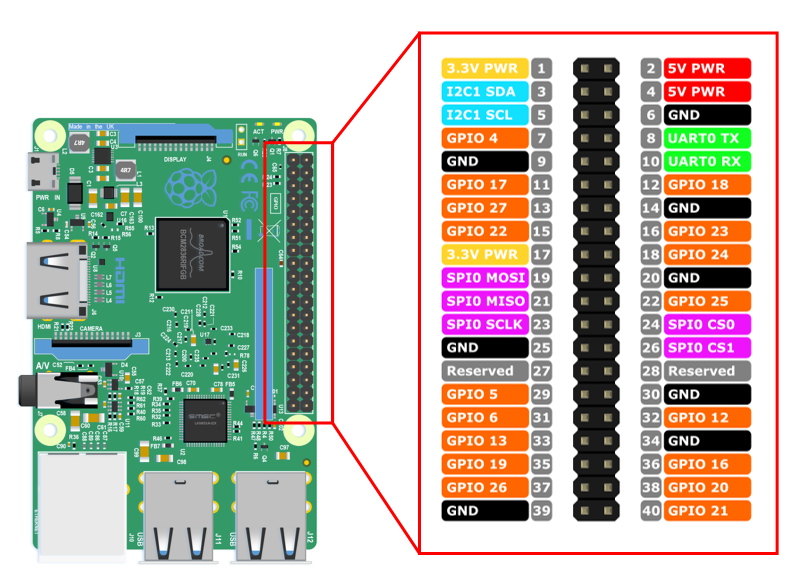
\includegraphics[width=0.8\textwidth]{pipins}
		\caption[EthernetPinbelegung]{Pinbelegung für die \gls{aussensprechstelle}}
		\label{fig:pipins}
	\end{center}
\end{figure}

\begin{figure}[htb!]
	\begin{center}
		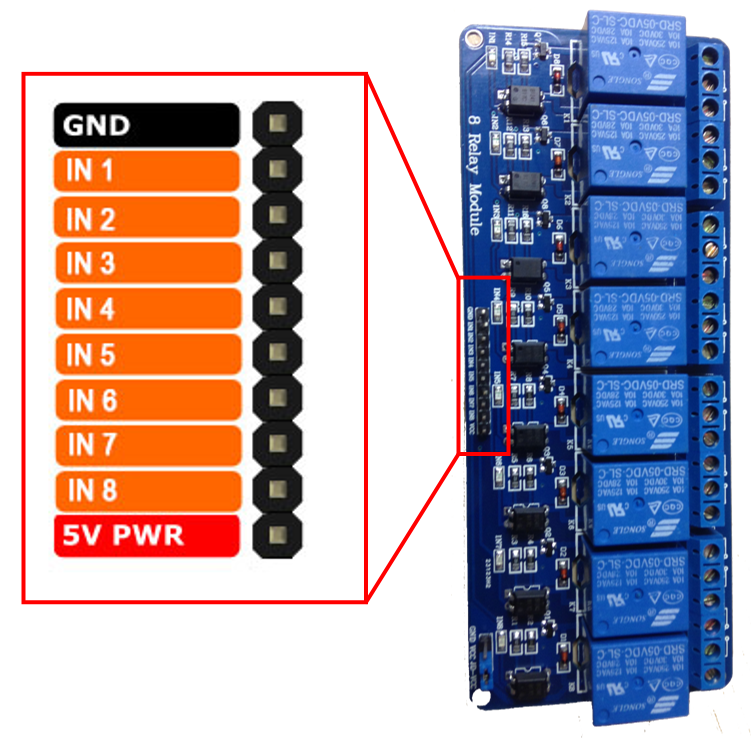
\includegraphics[width=0.55\textwidth]{boardpins}
		\caption[EthernetPinbelegung]{Pinbelegung für das Relais-Modul}
		\label{fig:boardpins}
	\end{center}
\end{figure}

\begin{table}[]
	\centering
	\label{my-label}
	\begin{tabular}{l|ll}
		\multicolumn{1}{r|}{} \textbf{Pi GPIO (PIN)} & \textbf{Relais IN (Board Nr)} & \textbf{Funktion}  \hspace{60pt}	\\ \hline
		GPIO4 (7)	&	IN1 (1)			& Gong WG.1			\\ \hline
		GPIO17 (11)	&	IN2 (1)			& Gong WG.2			\\ \hline
		GPIO27 (13)	&	IN3 (1)			& Gong WG.3			\\ \hline
		GPIO22 (15)	&	IN4 (1)			& Gong WG.4			\\ \hline
		GPIO5 (29)	&	IN5 (1)			& Gong WG.5			\\ \hline
		GPIO6 (31)	&	IN6 (1)			& Gong WG.6			\\ \hline
		GPIO13 (33)	&	IN7 (1)			& Gong WG.7			\\ \hline
		GPIO19 (35)	&	IN8 (1)			& Gong WG.8			\\ \hline
		GPIO18 (12)	&	IN1 (2)			& Türöffner Türe 1			\\ \hline
		GPIO23 (16)	&	IN2 (2)			& Türöffner Türe 2			\\ \hline
		GPIO24 (18)	&	IN3 (2)			& Türöffner Türe 3			\\ \hline
		GPIO25 (22)	&	IN4 (2)			& Türöffner Türe 4			\\ \hline
		GPIO12 (32)	&	IN5 (2)			& Türöffner Türe 5			\\ \hline
		GPIO16 (36)	&	IN6 (2)			& Türöffner Türe 6			\\ \hline
		GPIO20 (38)	&	IN7 (2)			& Türöffner Türe 7			\\ \hline
		GPIO21 (40)	&	IN8 (2)			& Türöffner Türe 8			\\ \hline
	\end{tabular}
	\caption{PIN-Zuweisung zwischen den Server und die Relais Module}
	\label{tbl:pinroutes}
\end{table}


\subsection{Aussensprechstelle}
\label{sec:chapterexample}

Bei der \gls{aussensprechstelle} wird auch eine Raspberry Pi eingesetzt. Hier sind mehrere Zusatzkomponenten notwendig. Die Speisung, wie oben schon erwähnt, erfolgt an dieser stelle über \gls{poe}, aus diesem Grund ist ein \gls{poe}-Splitter vorhanden.
\\
Für die Audiowiedergabe sind ein kleines Lautsprecher und ein Verstärker notwendeig. Die Chinch-Anschluss der Raspberry Pi hat eine zu niedrige Ausgangsleistung um den Lautsprecher direkt anschliessen zu können. 
\\
Die drei Schalter, die für die Bedienung der \gls{aussensprechstelle} notwendig sind, werden an die \gls{gpio}s der Raspberry PI angeschlossen. Die \cref{tbl:pinroutesdoor} zeigt die Pinbelegung.
\begin{table}[]
	\centering
	\label{my-label}
	\begin{tabular}{l|ll}
		\multicolumn{1}{r|}{} \textbf{Pi GPIO (PIN)} & \textbf{Schalter} & \textbf{Funktion} \hspace{60pt}	\\ \hline
		GPIO16 (36)	&	Schalter Links		&	Nach Links Scrollen	\\ \hline
		GPIO20 (38)	&	Schalter Mitte		&	Glocke läuten		\\ \hline
		GPIO21 (40)	&	Schalter Rechts		&	Nach Rechts Scrollen		\\ \hline
	\end{tabular}
	\caption{PIN-Zuweisung zwischen den Raspberry PI und die Schalter}
	\label{tbl:pinroutesdoor}
\end{table}

\subsubsection{Problemen}
Während der Zusammenstellung der Aussensprechstelle sind die erste unvorhergesehene Problemen aufgetaucht. Die Audiowiedergabe und Audioaufnahme stellten eine grössere Herausforderung als geplant dar.
\\
\\
\textbf{Audiowidergabe} 
\\
Die grösste Problematik bei der Audiowiedergabe besteht darin, dass die Massen des Raspberry Pi, der Verstärker und des Audio-Interface alle zusammen gekoppelt sind. Das führt zu Brummschleifen die wiederum Störsignale auf dem Audio-Ausgang erzeugen. Um das zu vermeiden wird ein Massentrennfilter an dieser Stelle eingesetzt.
\\
Die Störsignale sind nun fast komplett verschwunden, ein klein Hintergrundgeräusch ist aber immer noch vorhanden. Um dieses Problem umzugehen, wird ein zusätzliches Relay installiert, welche das Lautsprecher-Stromkreis unterbricht, wenn diese nicht verwendet wird.
\\
\\
\textbf{Das Mikrophon}
\\
Das Problem bei der Audioaufnahme liegt bei der Mikrophon selber. Die Raspberry Pi besitzt kein integriertes Audio-Input. Aus diesem Grund wurde ein \gls{usb}-Audio Interface verwendet. Es hat sich aber herausgestellt, dass nicht so einfach ist, kostengünstige und qualitatives \gls{usb} Mikrophone zu finden. Die meisten Produkten sind nicht für den Outdoor-Betrieb gedacht. Für unser Prototyp ist das eingesetzte Mikrophon völlig ausreichen. Für das Endprodukt sollte man hier noch etwas Zeit und Geld in der Evaluation ein besseres Mikrophon investieren.
\newpage